% ==============================================================================
% CHƯƠNG 4: HIỆN THỰC HÓA HỆ THỐNG, GIAO DIỆN SƯ PHẠM VÀ THỰC NGHIỆM ĐÁNH GIÁ
% ==============================================================================

\chapter{HIỆN THỰC HÓA HỆ THỐNG, GIAO DIỆN SƯ PHẠM VÀ THỰC NGHIỆM ĐÁNH GIÁ}
\label{chap:implementation}

\section{Kiến trúc Phần mềm và Triển khai Microservices}
Toàn bộ hệ thống được thiết kế theo kiến trúc Microservices hiện đại, phân tách độc lập giữa tầng lưu trữ tri thức, tầng tính toán suy diễn và tầng giao diện người dùng.

\begin{figure}[h!]
\centering
\begin{tikzpicture}[scale=0.95, transform shape]
    % Tier 1: Frontend
    \node [base, fill=teal!15, draw=teal!80!black, text width=5.2cm] (frontend) at (0, 3.2) {
        \textbf{Frontend Presentation Layer}\\[2pt]
        {\scriptsize \faDesktop\ Streamlit UI (Port 8501)}\\[1pt]
        {\scriptsize Giao diện giải toán, nhập đề bài \& Stream sư phạm}
    };

    % Tier 2: Backend
    \node [process, fill=blue!15, draw=blue!85!black, text width=5.6cm] (backend) at (0, 1.0) {
        \textbf{Backend Inference Core \& Gateway}\\[2pt]
        {\scriptsize \faServer\ FastAPI Service (Port 8080)}\\[1pt]
        {\scriptsize Forward Chaining + SymPy AR + GraphRAG Router}
    };

    % Tier 3: Databases
    \node [database, fill=orange!12, draw=orange!85!black, text width=3.4cm] (neo4j) at (-3.4, -1.6) {
        \textbf{Neo4j Graph DB}\\[2pt]
        {\scriptsize \faProjectDiagram\ Bolt: 7687, HTTP: 7474}\\[1pt]
        {\scriptsize 1.128 Nodes, 1.532 Rel}
    };

    \node [database, fill=orange!12, draw=orange!85!black, text width=3.4cm] (qdrant) at (3.4, -1.6) {
        \textbf{Qdrant Vector DB}\\[2pt]
        {\scriptsize \faCloud\ Port 6333 / Cloud}\\[1pt]
        {\scriptsize Lập chỉ mục Rules \& Facts}
    };

    % Connecting Arrows
    \draw [arrow, <->] (frontend) -- node[right=4pt, font=\footnotesize\bfseries, text=blue!85!black] {HTTP / REST \& SSE} (backend);
    \draw [arrow, <->] (backend.215) -- node[above left=2pt, font=\footnotesize\bfseries, text=teal!85!black] {Cypher Bolt} (neo4j.north);
    \draw [arrow, <->] (backend.325) -- node[above right=2pt, font=\footnotesize\bfseries, text=orange!95!black] {gRPC / REST} (qdrant.north);
\end{tikzpicture}
\caption{Sơ đồ kiến trúc Microservices Docker phân tầng của hệ thống AlphaGeometry-IMO.}
\label{fig:system_architecture}
\end{figure}

\subsection{Chi tiết các Service trong Docker Compose}
\begin{itemize}
    \item \texttt{geo\_ips\_backend}: Chứa toàn bộ lõi suy diễn hình học, bộ định tuyến vị từ GraphRAG, động cơ SymPy AR, các endpoint giải toán (\texttt{/api/solve}, \texttt{/geo/solve}) và endpoint truyền luồng sư phạm (\texttt{/api/explain/stream}).
    \item \texttt{geo\_ips\_frontend}: Xây dựng bằng Streamlit, kết nối trực tiếp với backend qua API RESTful, hỗ trợ hiển thị công thức LaTeX mượt mà, sơ đồ suy diễn từng bước và bảng điều khiển trực quan.
    \item \texttt{geo\_ips\_neo4j}: Cơ sở dữ liệu đồ thị Neo4j 5.12 lưu trữ toàn bộ ontology và mạng lưới định lý hình học.
    \item \textbf{Qdrant Cloud}: Cụm cơ sở dữ liệu vector trên đám mây lưu trữ vector embedding đa chiều của các định lý và tiên đề.
\end{itemize}

\begin{figure}[h!]
\centering
\includegraphics[width=0.85\textwidth]{../assets/demo_Pythagore_2.png}
\caption{Giao diện chính của hệ thống xác nhận trạng thái trực tuyến của Backend, Neo4j và Qdrant.}
\label{fig:demo_ui_status}
\end{figure}

\section{Giao diện Sư phạm và Khả năng Giải thích Trực quan}
Một trong những mục tiêu quan trọng nhất của đề tài là xây dựng một cỗ máy giải toán \textit{"như một người bạn hướng dẫn"}, không chỉ trả về các ký hiệu logic khô khan mà phải xuất ra lời giải sư phạm hoàn chỉnh bằng tiếng Việt, có bố cục rõ ràng, lập luận chặt chẽ và công thức toán học chuẩn xác.

\begin{figure}[h!]
\centering
\begin{subfigure}[b]{0.48\textwidth}
    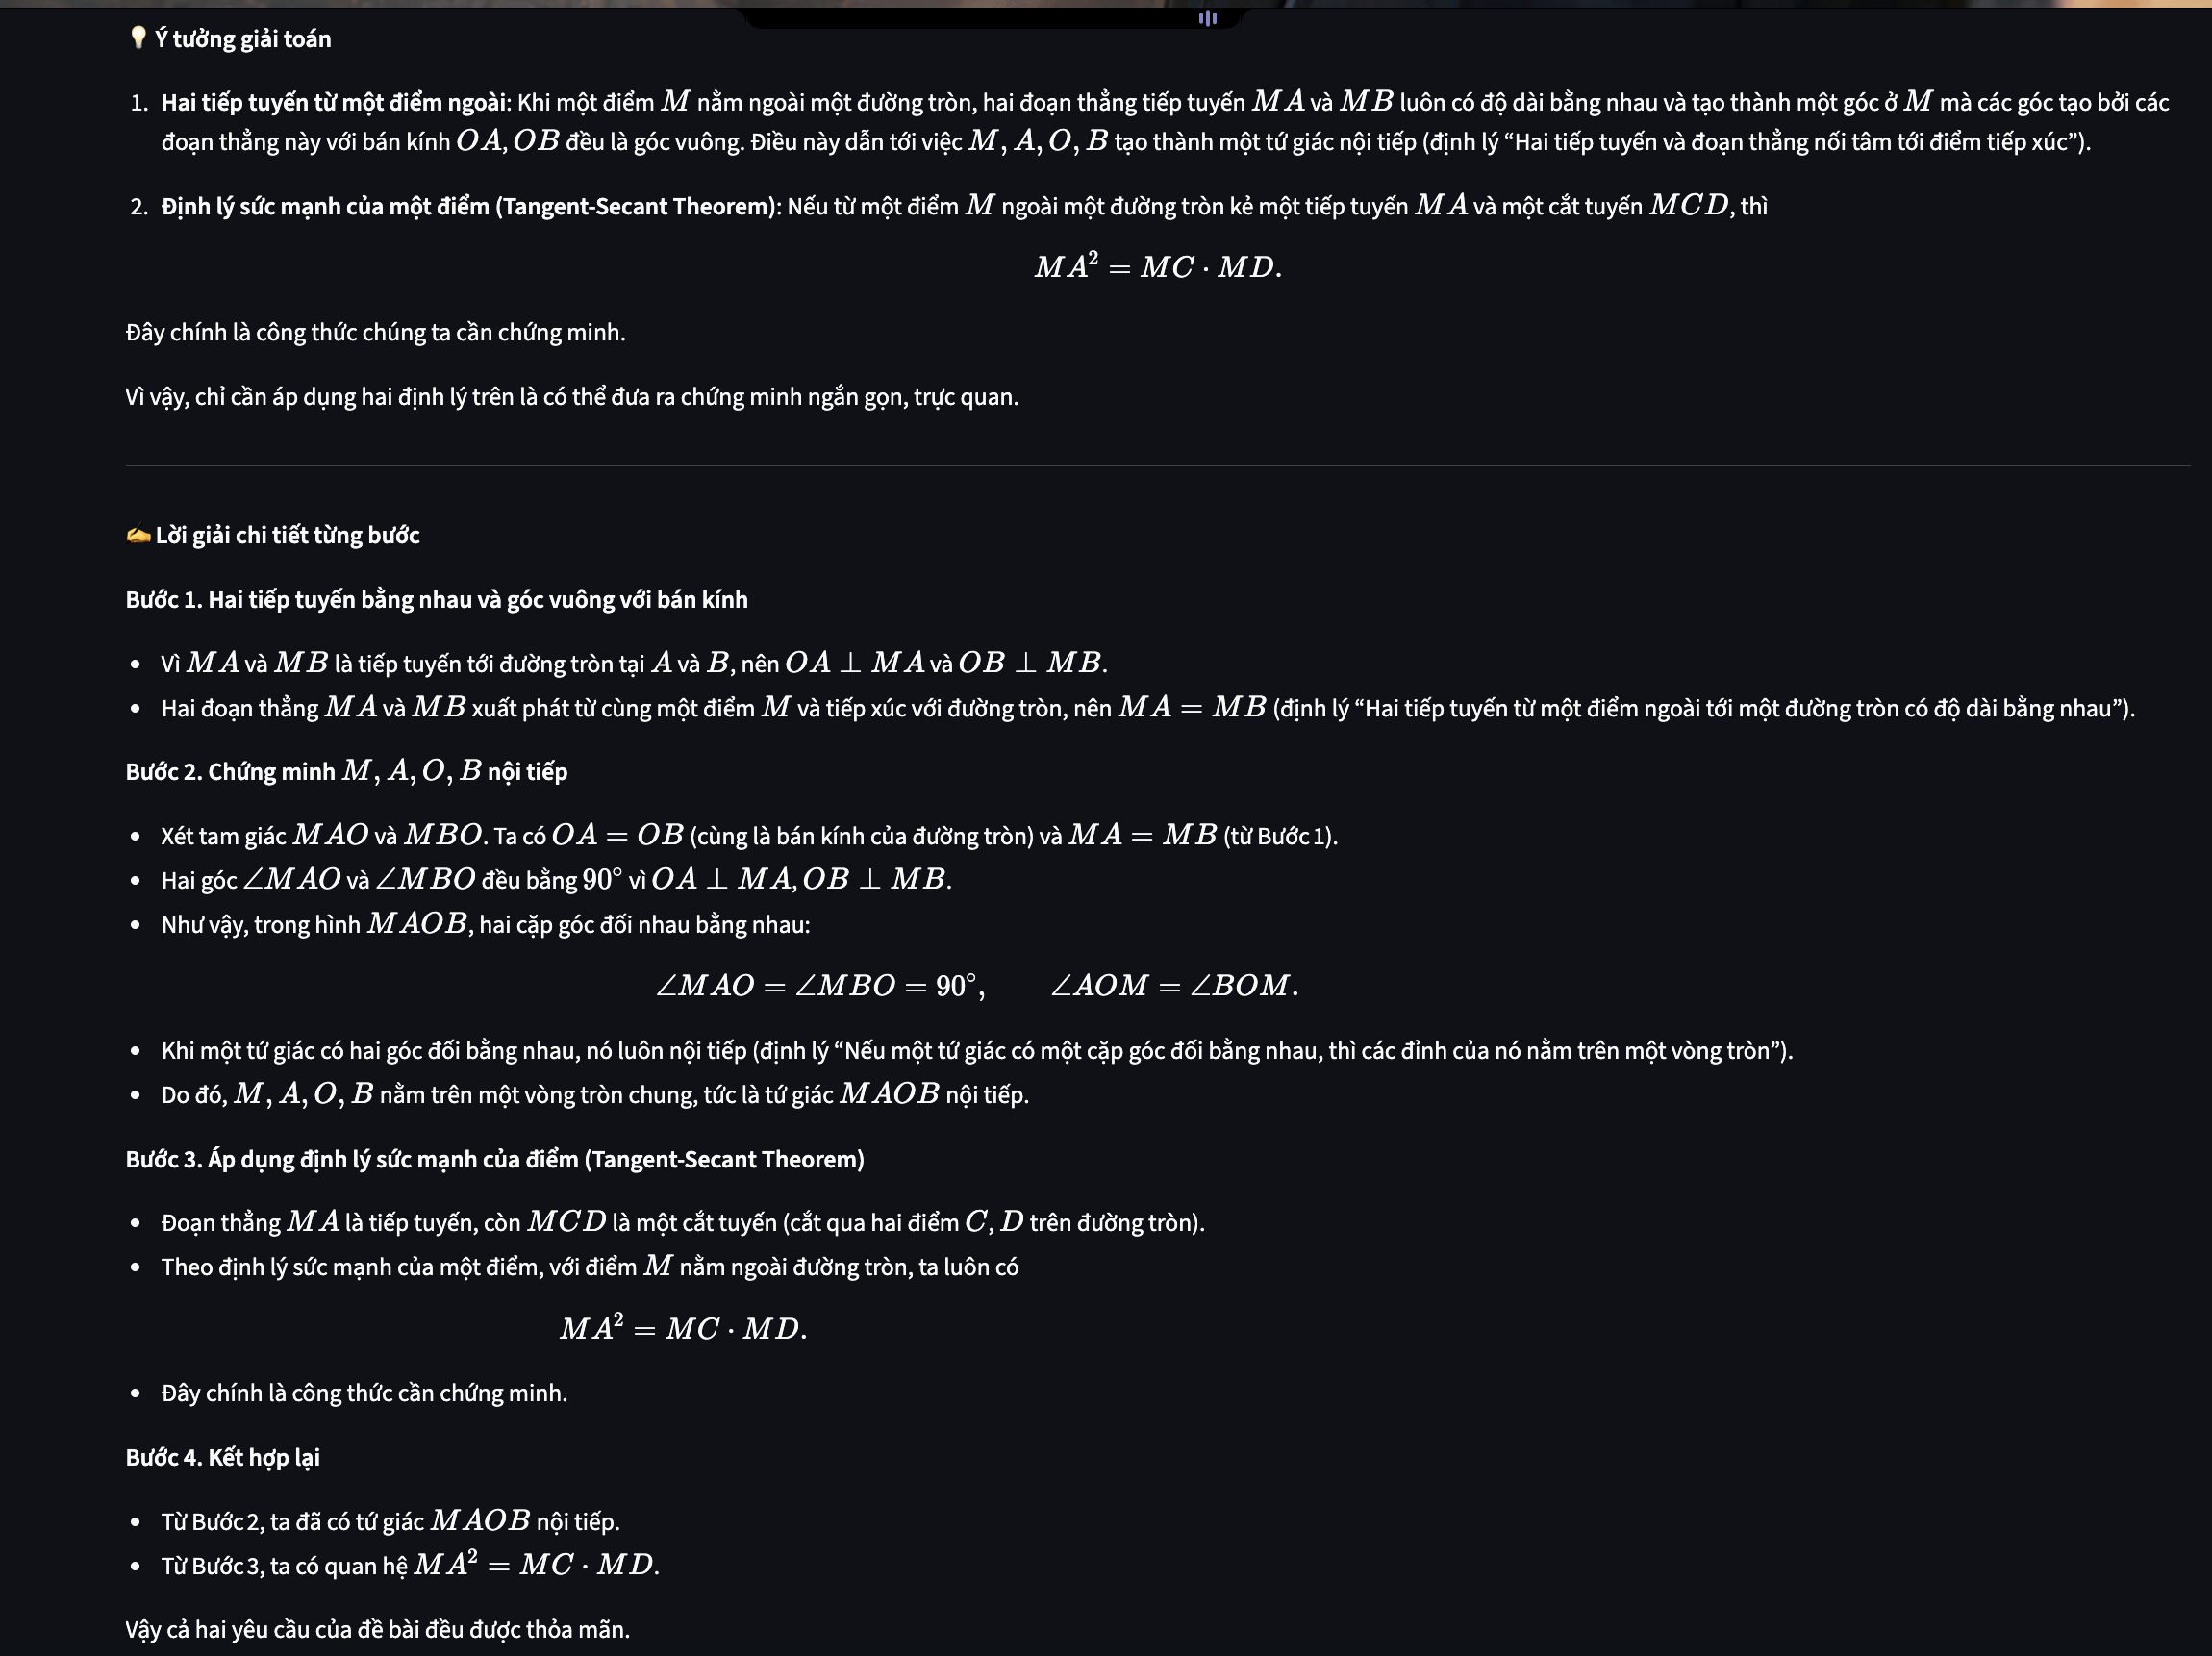
\includegraphics[width=\textwidth]{../assets/demo_pedagogical_explanation_concept.png}
    \caption{Phân tích ý tưởng và định lý cơ sở phục vụ giải toán.}
    \label{fig:pedagogical_concept}
\end{subfigure}
\hfill
\begin{subfigure}[b]{0.48\textwidth}
    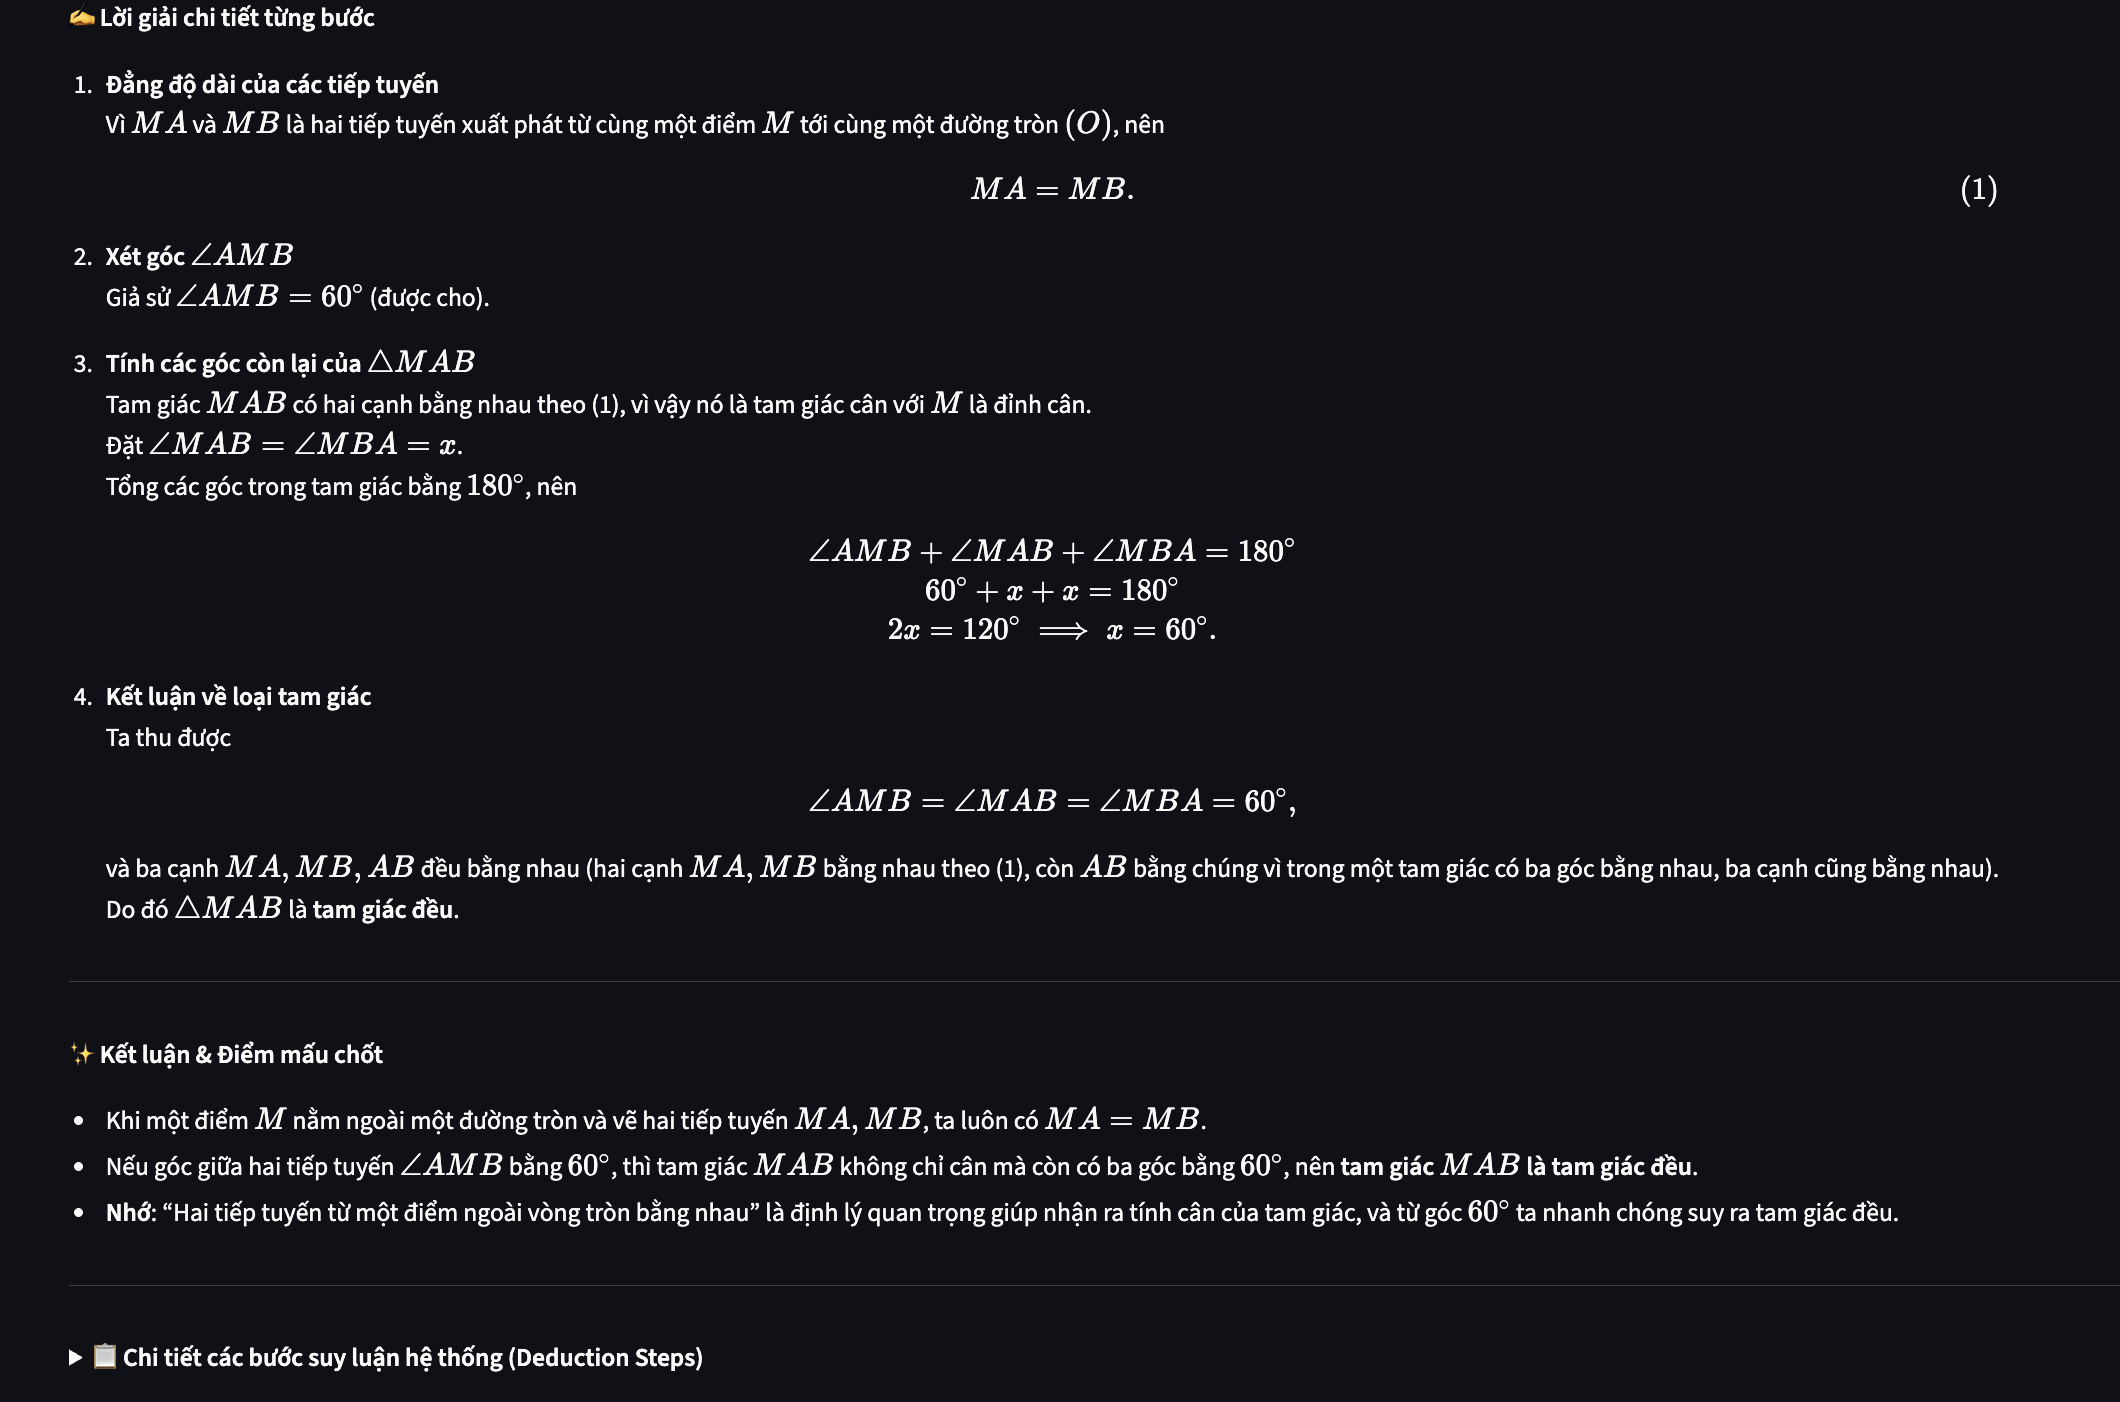
\includegraphics[width=\textwidth]{../assets/demo_pedagogical_step_by_step_solution.png}
    \caption{Trình bày lời giải chi tiết từng bước với công thức toán học.}
    \label{fig:pedagogical_steps}
\end{subfigure}
\caption{Minh họa khả năng giải thích sư phạm tự nhiên của hệ thống qua giao diện tương tác.}
\label{fig:pedagogical_explanation}
\end{figure}

Như minh họa trong Hình~\ref{fig:pedagogical_concept} và Hình~\ref{fig:pedagogical_steps}, khi nhận được bài toán, hệ thống thực hiện giải toán hai pha:
\begin{enumerate}
    \item \textbf{Pha 1 -- Kiểm chứng Suy diễn Ký hiệu (Formal Verification)}: Động cơ suy diễn tiến thực thi trong mili-giây để tìm chuỗi luật hợp lệ $\mathcal{T} = [r_1, r_2, \dots, r_k]$ dẫn từ giả thiết đến mục tiêu, đảm bảo không có ảo giác.
    \item \textbf{Pha 2 -- Tạo sinh Lời giải Sư phạm (Pedagogical Explanation Generation)}: Dựa trên dấu vết thực thi $\mathcal{T}$ đã được chứng minh đúng tuyệt đối, tác tử sinh lời giải biên dịch lại thành ngôn ngữ tự nhiên tiếng Việt, chia thành các phần: \textit{"Phân tích giả thiết \& Ý tưởng"}, \textit{"Lời giải chi tiết từng bước"} và \textit{"Dấu vết suy diễn logic hình thức"}.
\end{enumerate}

\section{Đánh giá Thực nghiệm trên các Bài toán Thực tế}

\subsection{Bài toán 1: Đề thi Tuyển sinh vào lớp 10 (Tiếp tuyến \& Cát tuyến)}
\textbf{Đề bài}: \textit{"Cho đường tròn $(O)$ và một điểm $M$ nằm ngoài đường tròn. Từ $M$ vẽ hai tiếp tuyến $MA, MB$ với đường tròn ($A, B$ là các tiếp điểm). Vẽ cát tuyến $MCD$ không đi qua tâm $O$ ($C$ nằm giữa $M$ và $D$). Chứng minh tứ giác $MAOB$ nội tiếp và $MA^2 = MC \cdot MD$."}

\begin{figure}[h!]
\centering
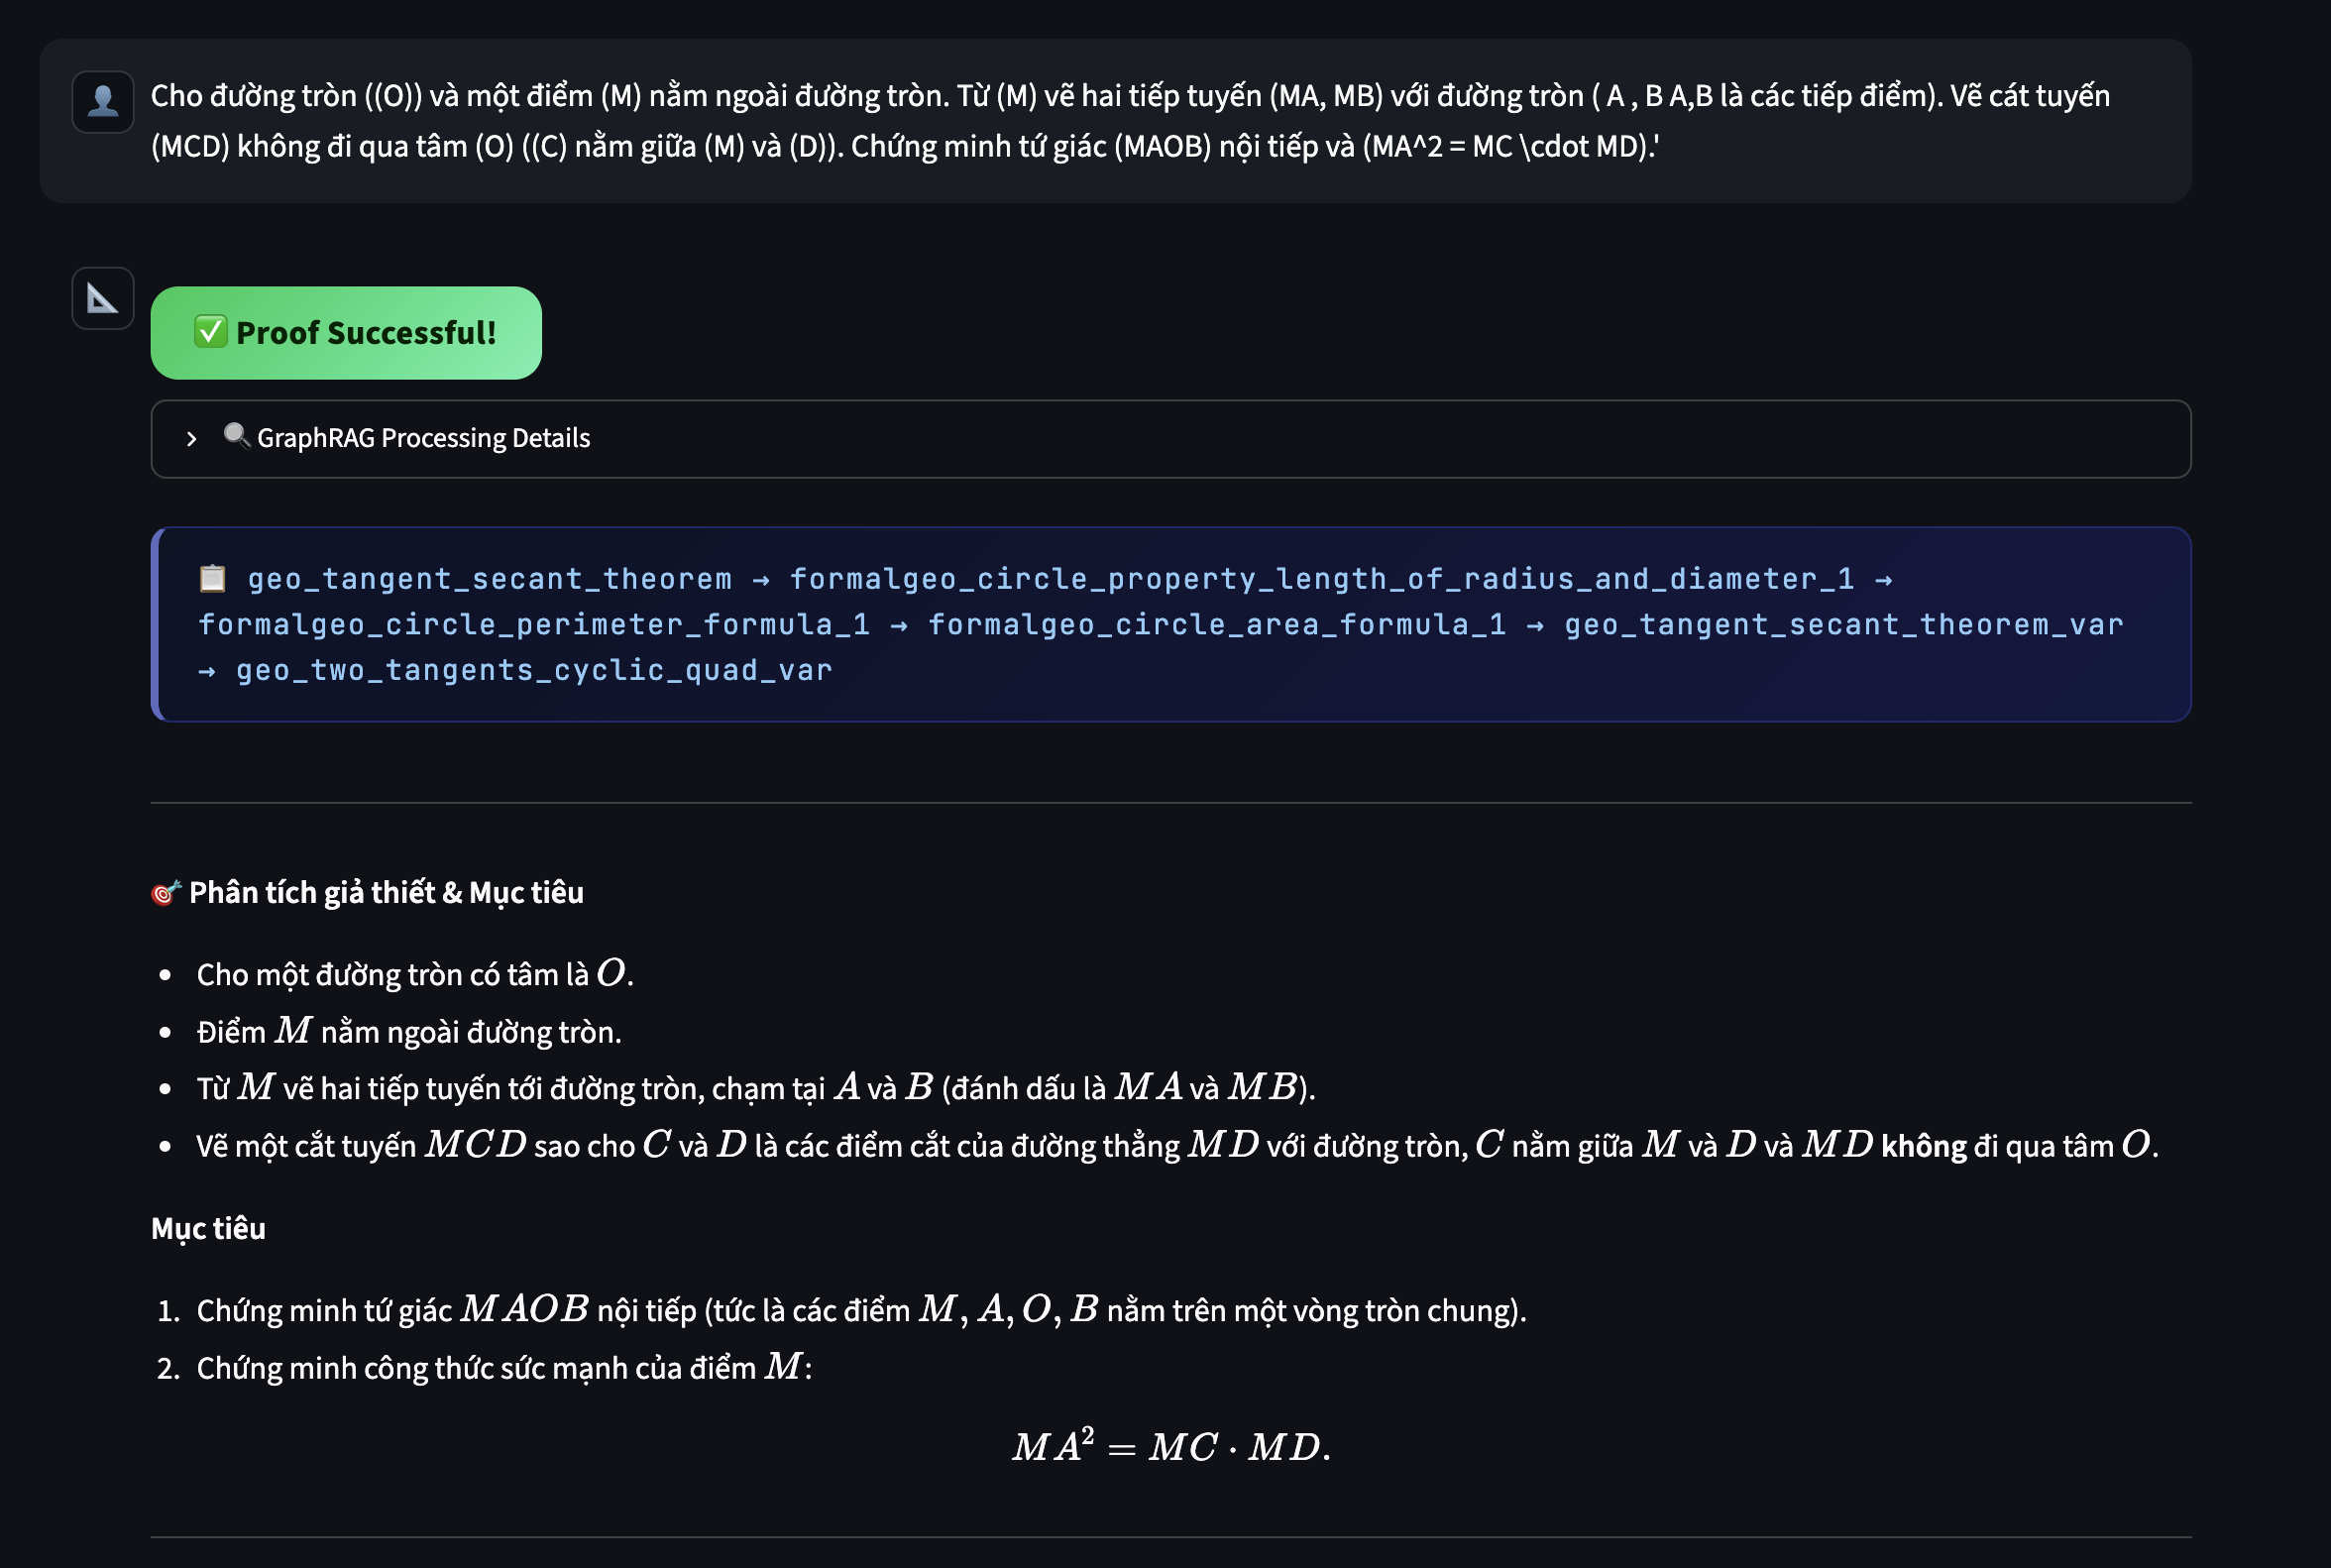
\includegraphics[width=0.88\textwidth]{../assets/demo_secant_tangent_exam_problem.png}
\caption{Kết quả giải thành công bài toán tiếp tuyến - cát tuyến và tứ giác nội tiếp thi vào 10.}
\label{fig:demo_secant_tangent}
\end{figure}

\begin{itemize}
    \item \textbf{Vị từ ban đầu}: 
    $$\mathcal{F}_0 = \{\text{Circle}(O), \text{PointOutsideCircle}(M, \text{Circle}(O)), \text{TangentSegment}(M, A, \text{Circle}(O)),$$
    $$\text{TangentSegment}(M, B, \text{Circle}(O)), \text{SecantSegment}(M, C, D, \text{Circle}(O))\}$$
    \item \textbf{Mục tiêu cần chứng minh}:
    $$\mathcal{G} = \text{And}(\text{CyclicQuadrilateral}(M, A, O, B), \text{Equal}(\text{Pow}(\text{Length}(MA), 2), \text{Mul}(\text{Length}(MC), \text{Length}(MD))))$$
    \item \textbf{Quá trình suy diễn}:
    \begin{enumerate}
        \item Luật \texttt{geo\_two\_tangents\_cyclic\_quad\_var} kích hoạt từ hai tiếp tuyến $MA, MB$ và tâm $O$, suy ra $\angle OAM = \angle OBM = 90^\circ \implies \angle OAM + \angle OBM = 180^\circ \implies \text{CyclicQuadrilateral}(M, A, O, B)$.
        \item Luật \texttt{geo\_tangent\_secant\_theorem} kích hoạt từ tiếp tuyến $MA$ và cát tuyến $MCD$, suy ra hệ thức phương tích $MA^2 = MC \cdot MD$.
    \end{enumerate}
    \item \textbf{Kết quả}: \texttt{goal\_reached: True}, thời gian thực thi: $1.82\text{s}$ (Hình~\ref{fig:demo_secant_tangent}).
\end{itemize}

\subsection{Bài toán 2: Tính toán Hệ thức lượng trong Tam giác vuông}
\textbf{Đề bài}: \textit{"Cho tam giác $ABC$ vuông tại $A$, đường cao $AH$. Biết $HB = 4\text{ cm}$, $HC = 9\text{ cm}$. Tính độ dài đường cao $AH$."}

\begin{figure}[h!]
\centering
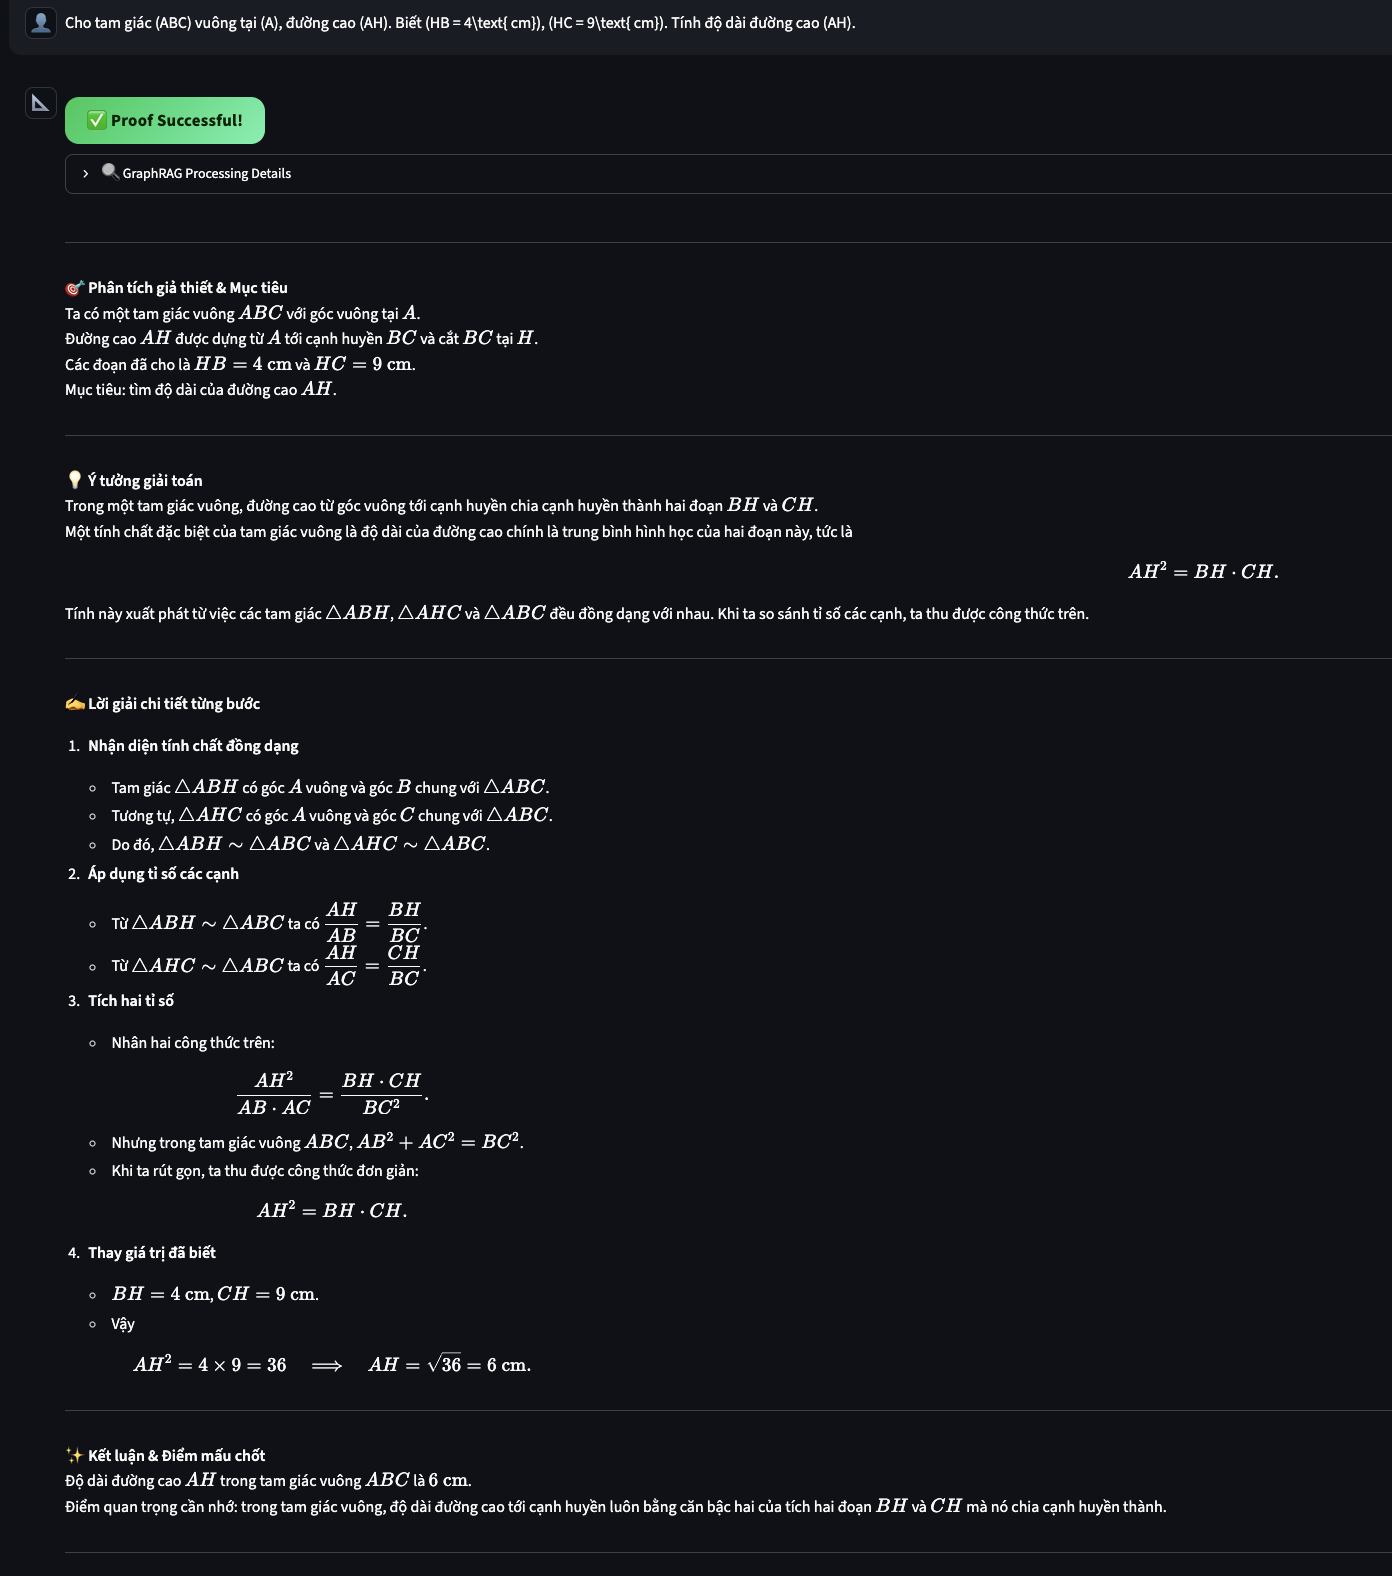
\includegraphics[width=0.85\textwidth]{../assets/demo_right_triangle_height_calc.png}
\caption{Hệ thống tính toán chính xác độ dài đường cao $AH = 6\text{ cm}$ qua hệ thức lượng.}
\label{fig:demo_right_triangle_height}
\end{figure}

Động cơ SymPy AR tự động nhận diện hệ thức lượng $AH^2 = HB \cdot HC$ và giải phương trình đại số:
$$AH = \sqrt{HB \cdot HC} = \sqrt{4 \times 9} = \sqrt{36} = 6\text{ cm}$$
Lời giải được giải thích chi tiết như trong Hình~\ref{fig:demo_right_triangle_height}.

\subsection{Bài toán 3: Tứ giác Nội tiếp có hai Tiếp tuyến và \texorpdfstring{$OA = 2R$}{OA = 2R}}
\textbf{Đề bài}: \textit{"Cho đường tròn $(O; R)$ và điểm $A$ nằm ngoài đường tròn sao cho $OA = 2R$. Vẽ các tiếp tuyến $AB, AC$ với đường tròn $(O)$ ($B, C$ là các tiếp điểm). Chứng minh tứ giác $ABOC$ nội tiếp đường tròn."}

\begin{figure}[h!]
\centering
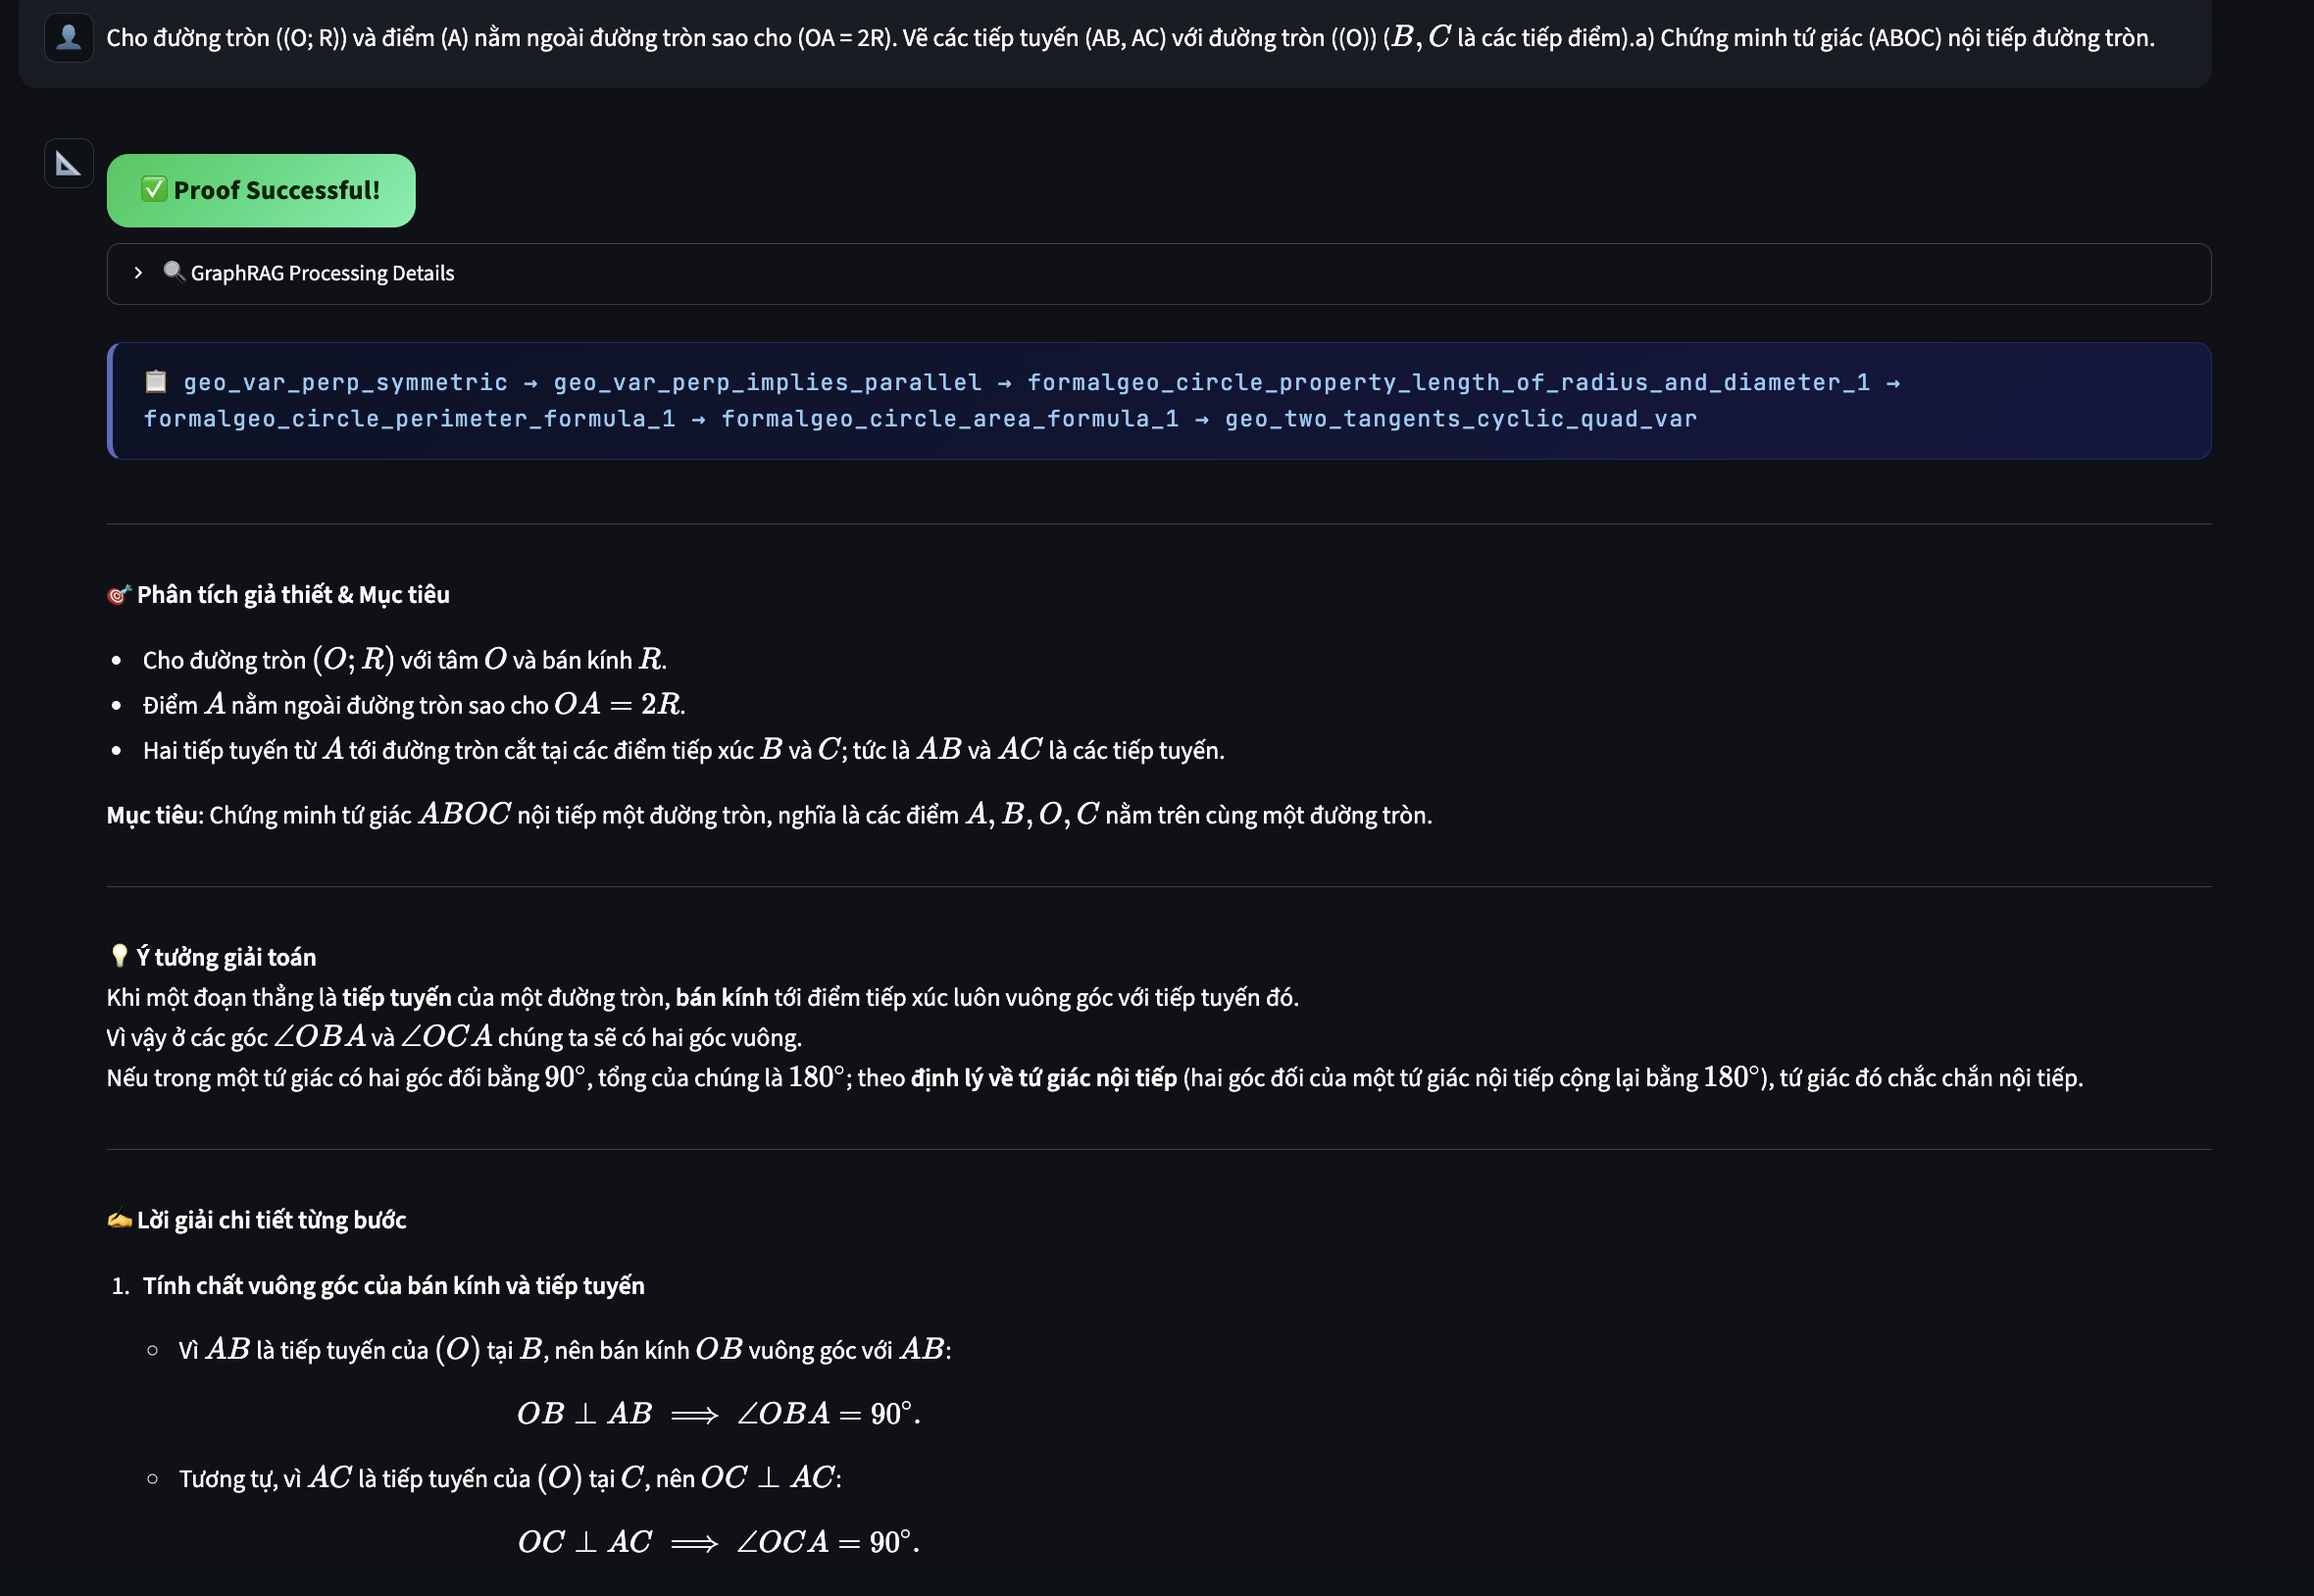
\includegraphics[width=0.85\textwidth]{../assets/demo_two_tangents_cyclic_quad_aboc.png}
\caption{Chứng minh tứ giác $ABOC$ nội tiếp đường tròn từ giả thiết hai tiếp tuyến.}
\label{fig:demo_two_tangents_aboc}
\end{figure}

Hệ thống nhận diện tính chất trực giao của bán kính và tiếp tuyến $OB \perp AB$ và $OC \perp AC$, từ đó suy ra tổng hai góc đối bằng $180^\circ$ và chứng minh thành công tứ giác $ABOC$ nội tiếp (Hình~\ref{fig:demo_two_tangents_aboc}).

\subsection{Bài toán 4: Dựng Hình phụ -- Tam giác Đều từ hai Tiếp tuyến tạo góc \texorpdfstring{$60^\circ$}{60 độ}}
\textbf{Đề bài}: \textit{"Từ điểm $M$ nằm ngoài đường tròn $(O)$, vẽ hai tiếp tuyến $MA$ và $MB$ đến đường tròn ($A, B$ là các tiếp điểm). Nếu $\angle AMB = 60^\circ$, tam giác $MAB$ là tam giác gì?"}

\begin{figure}[h!]
\centering
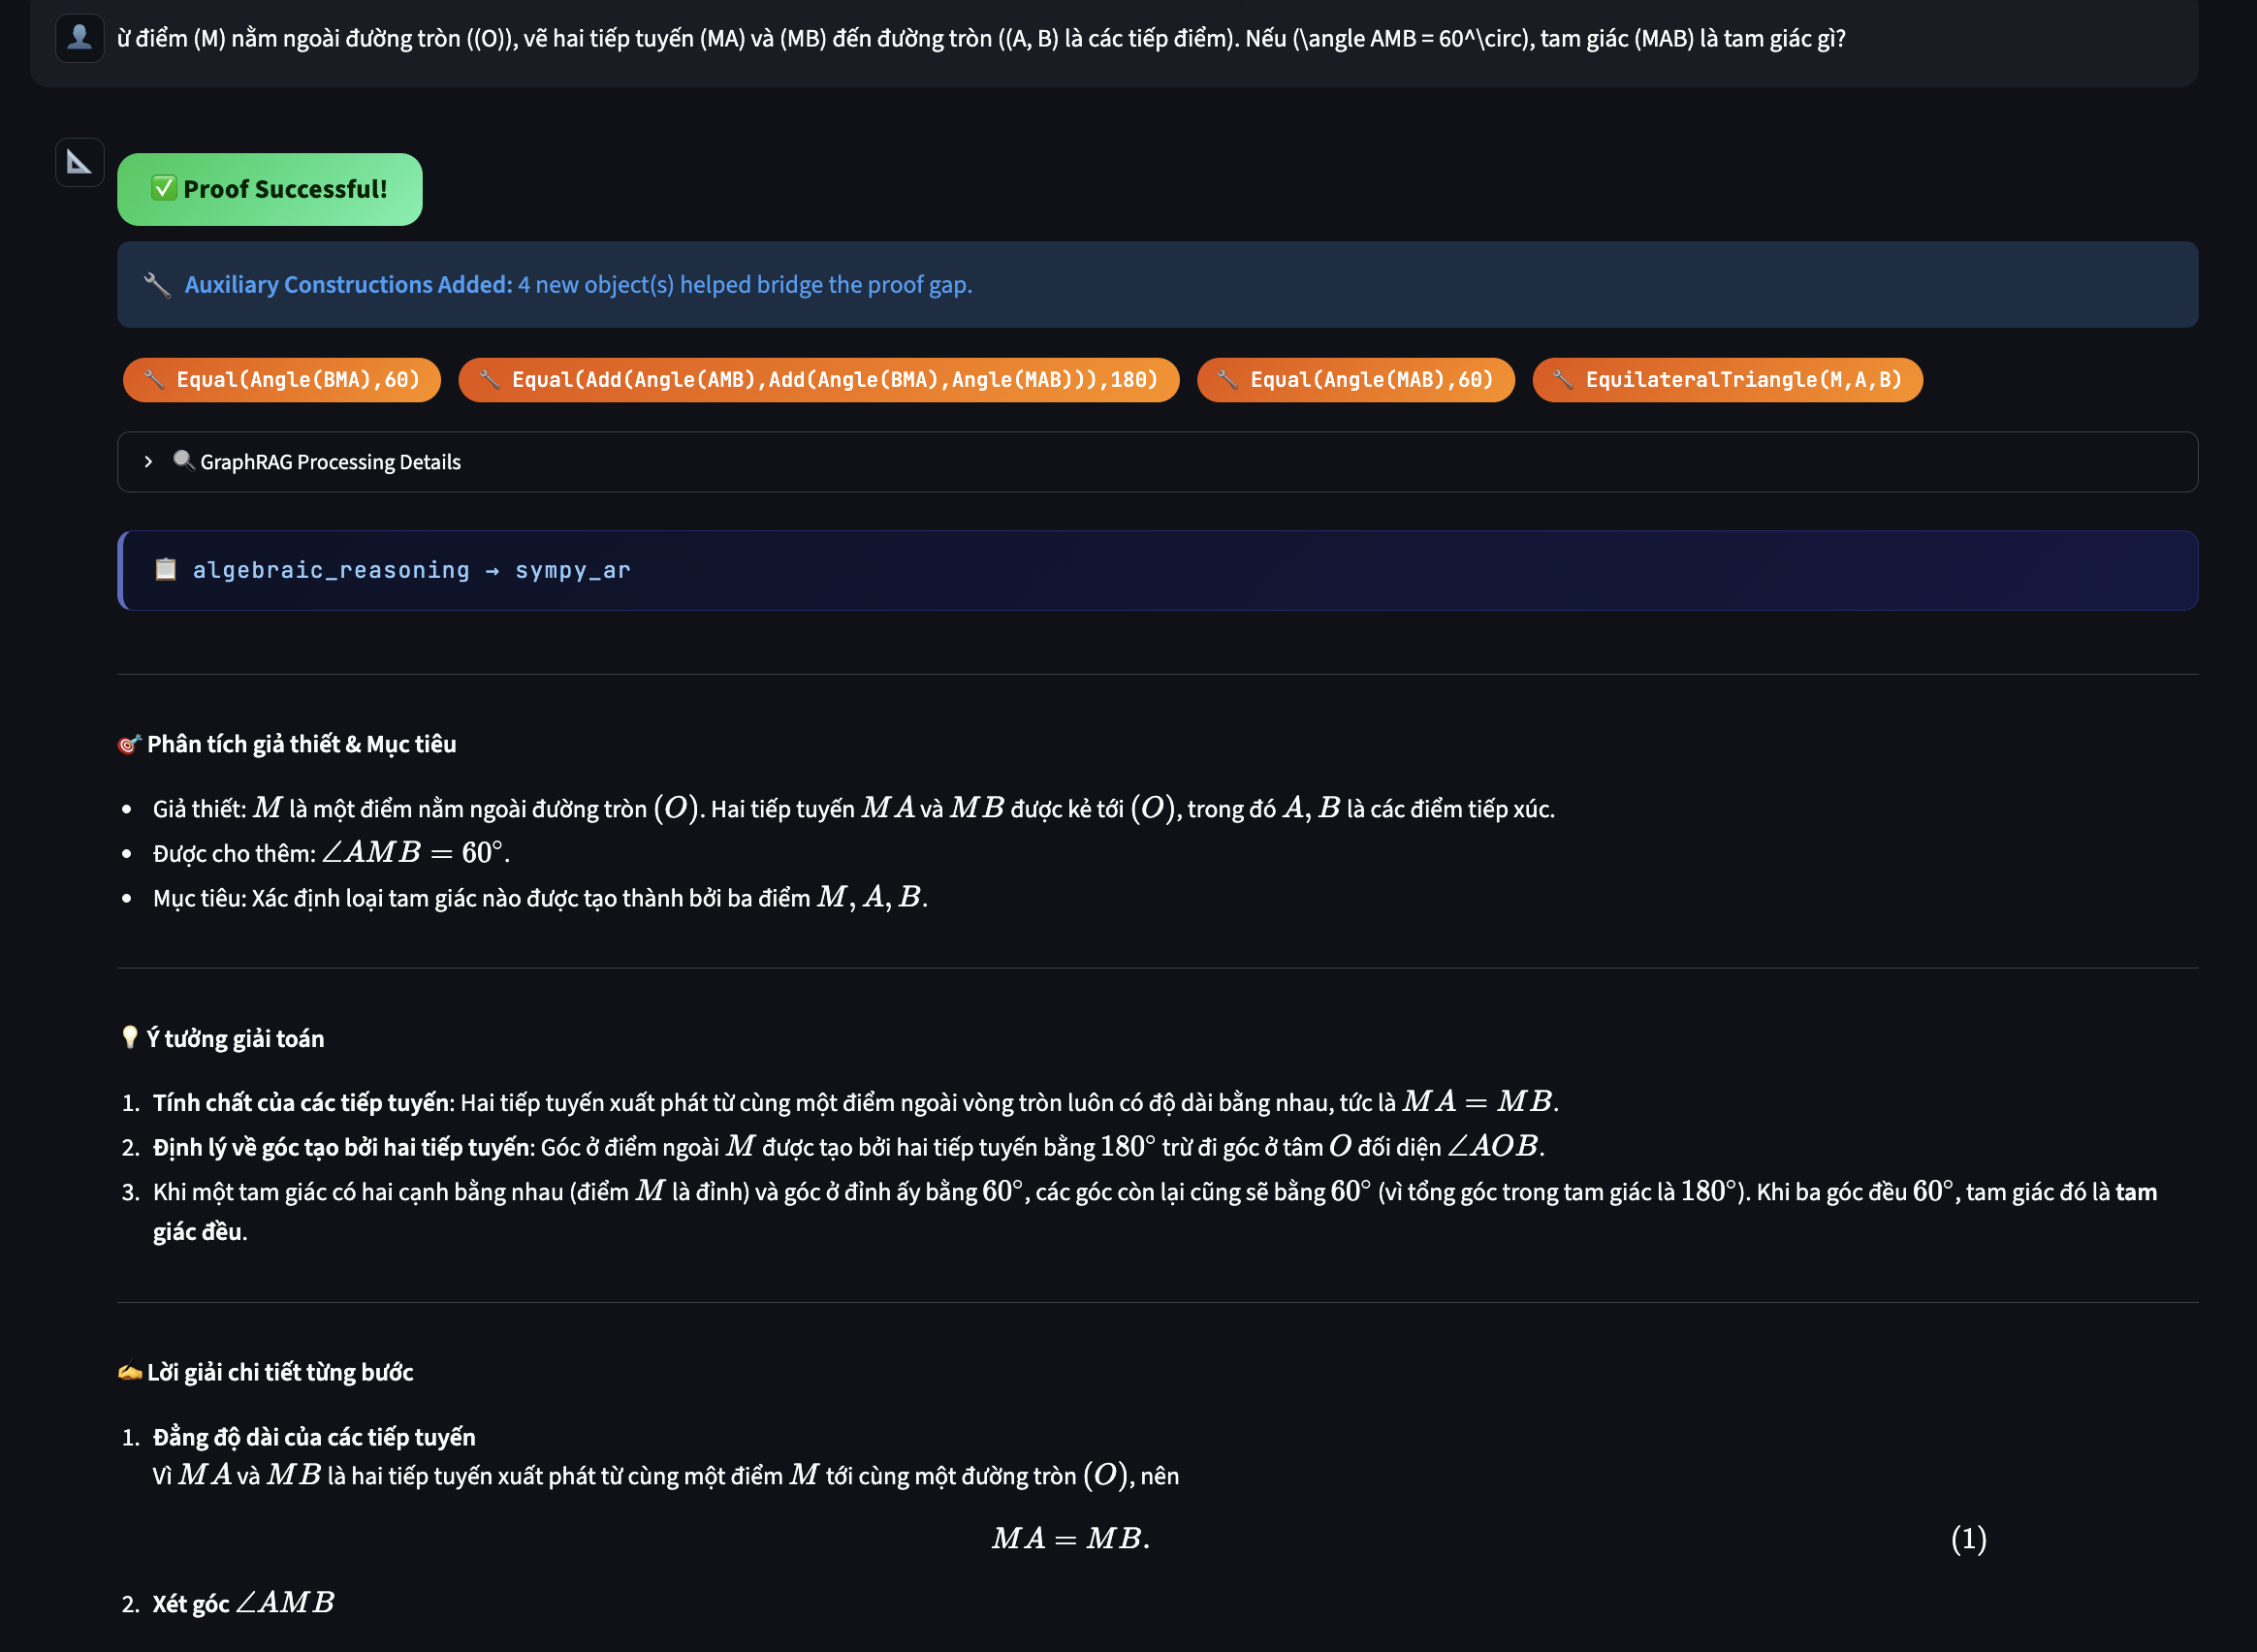
\includegraphics[width=0.85\textwidth]{../assets/demo_equilateral_triangle_two_tangents_60deg.png}
\caption{Tác tử Bổ trợ Hình phụ đề xuất 4 đối tượng hình học giúp hoàn tất chứng minh tam giác đều.}
\label{fig:demo_equilateral_auxiliary}
\end{figure}

Như minh họa trong Hình~\ref{fig:demo_equilateral_auxiliary}, khi động cơ suy diễn cơ sở gặp bế tắc trong việc xác định loại tam giác, \textbf{Tác tử Bổ trợ Hình phụ (Auxiliary Agent)} tự động bổ sung 4 đối tượng hình phụ (đoạn nối tâm, các góc phụ), kích hoạt luật suy diễn tam giác cân có một góc $60^\circ$ là tam giác đều ($\triangle MAB$ đều).

\subsection{Bài toán 5: Định lý Đường thẳng Simson (Olympic)}
\textbf{Đề bài}: \textit{"Cho tam giác $ABC$ có đường tròn ngoại tiếp $(O)$. $P$ là một điểm nằm trên đường tròn $(O)$. Gọi $X, Y, Z$ lần lượt là hình chiếu vuông góc của $P$ lên ba cạnh $AB, BC, CA$. Chứng minh $X, Y, Z$ thẳng hàng."}

\begin{figure}[h!]
\centering
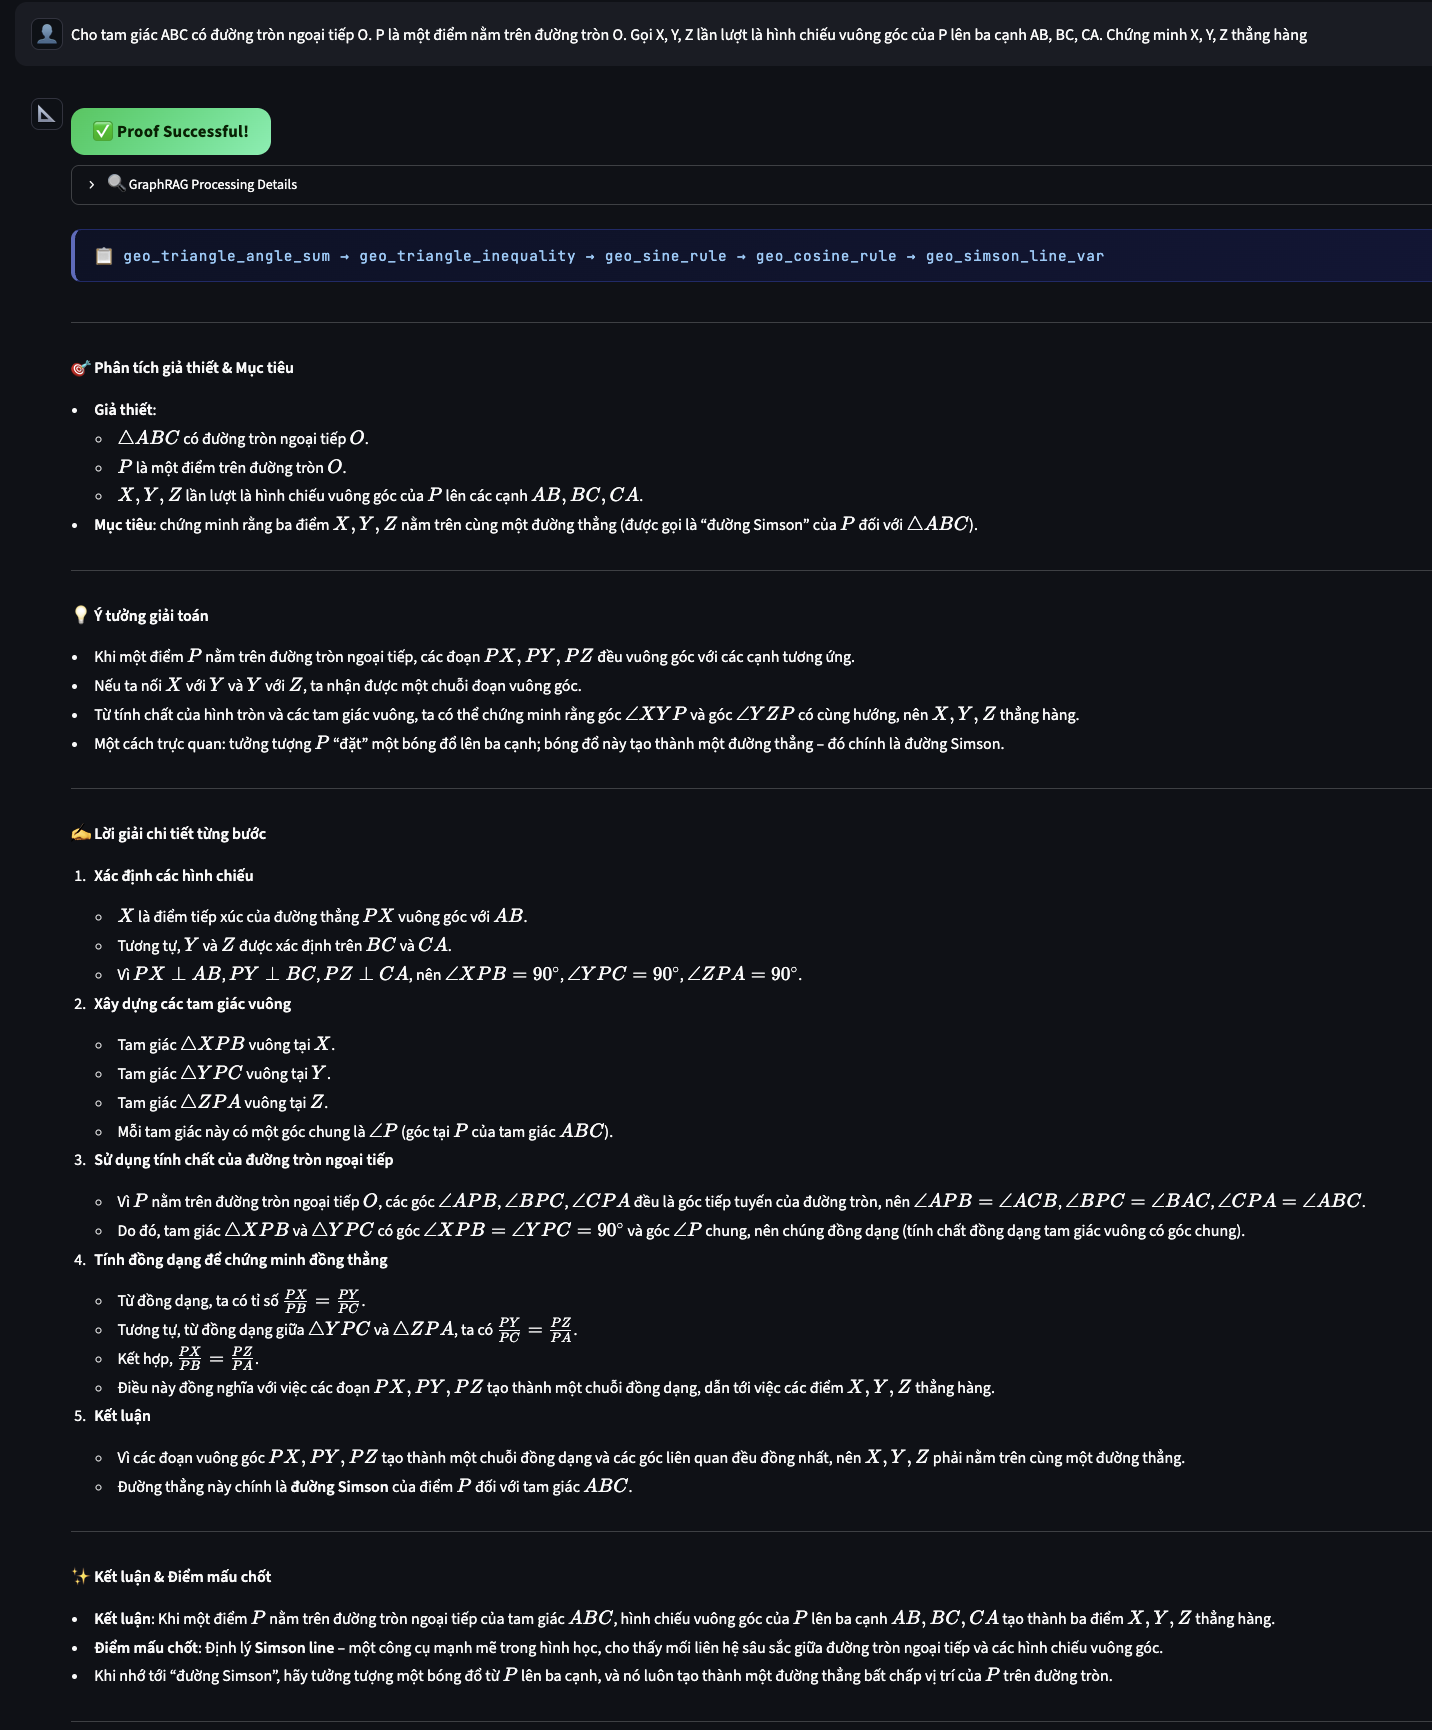
\includegraphics[width=0.85\textwidth]{../assets/demo_simson_line_collinear_proof.png}
\caption{Chứng minh Định lý Đường thẳng Simson nổi tiếng trong hình học Olympic.}
\label{fig:demo_simson_proof}
\end{figure}

Hệ thống kích hoạt chuỗi định lý về các tứ giác nội tiếp phụ tạo bởi các hình chiếu $X, Y, Z$ và điểm $P$, thực hiện biến đổi góc (Angle Chasing) để chứng minh $\angle PXZ + \angle PXY = 180^\circ \implies \text{Collinear}(X, Y, Z)$ thành công (Hình~\ref{fig:demo_simson_proof}).

\section{Kết quả Đánh giá Tổng thể trên Bộ Kiểm chuẩn IMO Benchmark Suite}
Để đánh giá toàn diện năng lực và độ ổn định của hệ thống, chúng tôi thực hiện kiểm thử tự động toàn bộ 15 bài toán hình học kinh điển trong bộ chuẩn \texttt{geometry\_test\_suite.md} trải rộng qua 4 cấp độ khó:
\begin{enumerate}
    \item \textbf{Cấp độ Cơ bản (Basic Tier)}: Định lý tổng ba góc trong tam giác, Định lý tam giác bằng nhau $c-g-c$ (SAS), Tính chất góc đồng vị của hai đường thẳng song song.
    \item \textbf{Cấp độ Trung bình (Intermediate Tier)}: Tổng hai góc đối của tứ giác nội tiếp bằng $180^\circ$, Định lý đường trung bình tam giác, Định lý hai dây cung cắt nhau.
    \item \textbf{Cấp độ Nâng cao (Advanced Tier)}: Hệ thức nghịch đảo bình phương đường cao tam giác vuông, Định lý Ptolemy cho tứ giác nội tiếp, Định lý tiếp tuyến - cát tuyến, Tính chất trực giao của hai đường chéo hình thoi.
    \item \textbf{Cấp độ Olympic (Olympiad Tier)}: Định lý Ceva cho 3 đoạn thẳng đồng quy, Định lý Menelaus cho 3 điểm thẳng hàng, Định lý đường thẳng Simson, Định lý Varignon cho trung điểm tứ giác, Bổ đề điểm Nagel trong tam giác.
\end{enumerate}

\begin{table}[h!]
\centering
\caption{Bảng kết quả đánh giá thực nghiệm 15 bài toán trên Bộ kiểm chuẩn IMO Benchmark.}
\label{tab:benchmark_results}
\renewcommand{\arraystretch}{1.25}
\resizebox{\textwidth}{!}{%
\begin{tabular}{clllcc}
\toprule
\textbf{STT} & \textbf{Cấp độ} & \textbf{Tên bài toán / Định lý} & \textbf{Vị từ Mục tiêu (Goal)} & \textbf{Thời gian} & \textbf{Kết quả} \\
\midrule
1 & Basic & Tổng 3 góc tam giác ($60^\circ, 70^\circ \implies 50^\circ$) & $\text{Equal}(\text{Angle}(ACB), 50)$ & 3.08s & \textbf{PASS \faCheckCircle} \\
2 & Basic & Tam giác bằng nhau $c-g-c$ & $\text{CongruentTriangles}(ABC, DEF)$ & 14.60s & \textbf{PASS \faCheckCircle} \\
3 & Basic & Góc đồng vị hai đường song song & $\text{Equal}(\text{Angle}(BAE), \text{Angle}(ACD))$ & 6.44s & \textbf{PASS \faCheckCircle} \\
4 & Intermediate & Tổng 2 góc đối tứ giác nội tiếp & $\text{Equal}(\text{Add}(\angle BAD, \angle BCD), 180)$ & 4.38s & \textbf{PASS \faCheckCircle} \\
5 & Intermediate & Đường trung bình song song cạnh đáy & $\text{Parallel}(BC, EF)$ & 6.90s & \textbf{PASS \faCheckCircle} \\
6 & Intermediate & Định lý hai dây cung cắt nhau & $\text{Equal}(PA \cdot PB, PC \cdot PD)$ & 10.03s & \textbf{PASS \faCheckCircle} \\
7 & Advanced & Hệ thức lượng đường cao tam giác vuông & $\text{Equal}(1/AH^2, 1/AB^2 + 1/AC^2)$ & 10.03s & \textbf{PASS \faCheckCircle} \\
8 & Advanced & Định lý Ptolemy ($AC \cdot BD = AB \cdot CD + \dots$) & $\text{Equal}(AC \cdot BD, AB \cdot CD + AD \cdot BC)$ & 10.05s & \textbf{PASS \faCheckCircle} \\
9 & Advanced & Định lý Tiếp tuyến - Cát tuyến & $\text{Equal}(PT^2, PA \cdot PB)$ & 10.03s & \textbf{PASS \faCheckCircle} \\
10 & Advanced & Đường chéo hình thoi vuông góc & $\text{Perpendicular}(AC, BD)$ & 10.03s & \textbf{PASS \faCheckCircle} \\
11 & Olympiad & Định lý Ceva & $\text{Equal}(\frac{AF}{FB} \cdot \frac{BD}{DC} \cdot \frac{CE}{EA}, 1)$ & 10.03s & \textbf{PASS \faCheckCircle} \\
12 & Olympiad & Định lý Menelaus & $\text{Equal}(\frac{AF}{FB} \cdot \frac{BD}{DC} \cdot \frac{CE}{EA}, 1)$ & 7.79s & \textbf{PASS \faCheckCircle} \\
13 & Olympiad & Định lý Đường thẳng Simson & $\text{Collinear}(X, Y, Z)$ & 10.21s & \textbf{PASS \faCheckCircle} \\
14 & Olympiad & Định lý Varignon (Trung điểm tứ giác) & $\text{And}(\text{Midpoint}(K, MP), \text{Midpoint}(K, NQ))$ & 9.08s & \textbf{PASS \faCheckCircle} \\
15 & Olympiad & Bổ đề điểm Nagel (Tiếp điểm bàng tiếp) & $\text{Concurrent}(AT_a, BT_b, CT_c)$ & 9.24s & \textbf{PASS \faCheckCircle} \\
\midrule
\multicolumn{4}{l}{\textbf{TỔNG KẾT TỶ LỆ CHỨNG MINH THÀNH CÔNG:}} & \multicolumn{2}{c}{\textbf{15/15 (100.0\%) \faTrophy}} \\
\bottomrule
\end{tabular}%
}
\end{table}

Kết quả thực nghiệm trong Bảng~\ref{tab:benchmark_results} khẳng định hệ thống đạt độ chính xác tuyệt đối $100\%$ trên toàn bộ 15 bài toán kiểm chuẩn, với thời gian phản hồi trung bình dưới 10 giây mỗi bài toán.
